\documentclass[conference]{style/IEEEtran}  
\IEEEoverridecommandlockouts
% The preceding line is only needed to identify funding in the first footnote. If that is unneeded, please comment it out.
\usepackage{cite}
\usepackage{amsmath,amssymb,amsfonts}
\usepackage{algorithmic}
\usepackage[dvipdfmx]{graphicx,color}
\usepackage{textcomp}
\usepackage{xcolor}

\def\BibTeX{{\rm B\kern-.05em{\sc i\kern-.025em b}\kern-.08em
    T\kern-.1667em\lower.7ex\hbox{E}\kern-.125emX}}

\usepackage{bm}

%% \usepackage{geometry}
%% \usepackage[dvipdfmx]{graphicx}
%% \usepackage{booktabs}
%% \usepackage[dvipdfmx]{color}
%% \usepackage{amsmath,amssymb}
%% \usepackage{url}
%% \usepackage{listings,jlisting}
%% \usepackage{here}
%% \usepackage[dvipdfmx]{hyperref}


%% \usepackage{ascmac}

%% \geometry{
%%   left=15mm,
%%   top=15mm,
%%   right=15mm,
%%   bottom=15mm
%%  }
%% %
%% \renewcommand{\lstlistingname}{コード}
%% %


%
\begin{document}

\title{Vibration extraction FPGA system for stabilization of surgical instruments under a microscope in an actual experiment.}


%% \author{
%% Authors name are omitted for double blind review  
%% }

\author{
  Kengo Yanagihara\IEEEauthorrefmark{1},
  %% Keizo Yamashita\IEEEauthorrefmark{1},
  Taito Manabe\IEEEauthorrefmark{1}, 
  Yuichiro Shibata\IEEEauthorrefmark{1},\\
  %% Masakatsu Tanaka\IEEEauthorrefmark{2},
  Shunji Moromugi\IEEEauthorrefmark{2}, 
  Masafumi Uematsu\IEEEauthorrefmark{3},
  %% Takashi Kitaoka\IEEEauthorrefmark{3},
  \\
  \IEEEauthorrefmark{1}Graduate School of Engineering, Nagasaki University, 1--14 Bunkyo-machi, Nagasaki-shi, Nagasaki 852-8256,Japan\\
  \IEEEauthorrefmark{2}Graduate School of Science and Engineering, Chuo University, 1--13--27 Kasuga, Bunkyo-ku, Tokyo 112-8551,Japan\\
  \IEEEauthorrefmark{3}Ophthalmology, Nagasaki University Hospital, 1--7--1 Sakamoto, Nagasaki-shi, Nagasaki 852-8501,Japan\\
  E-mail: \IEEEauthorrefmark{1}\{kengo,manabe,shibata\}@pca.cis.nagasaki-u.ac.jp
}


\maketitle

\begin{abstract}
  %% 本論文では、眞邊らが提案したマイクロサージェリーにおける振戦振動の抑制を実現するために提案した
  %% リアルタイム振動抽出システムの評価を行う。
  %% 実機動作すつ振動抽出システムの振動抽出精度、振動抑制の評価を行うため、3つの実験を行った。
  %% まずはじめに、内視鏡手術の模擬映像を用いた振動抽出実験を行い、
  %% システムの振動抽出精度を評価した。
  %% また、複数のシステムパラメータの値で実験を行い抽出精度への影響度を評価した。その結果、一部のパラメータを変更することで振動の抽出精度が向上することがわかった。
  %% 次に、振動抽出システムと逆位相波加振装置を接続し、加振実験を行った。
  %% 振動抽出システムの出力値どおりに加振できるか、加振精度の評価を行った。
  %% その結果、加振振動には意図しない高周波数成分が含まれており、精度良く加振をできているとは言えない
  %% 結果だった。
  %% 最後に、振戦振動を再現することができる振戦再現装置を用いて、振戦抑制実験を行った。
  %% 抑制結果は加振振動の遅延や精度の影響もあり振戦振動の周波数帯域以外の振動が増加してしまっていたが、
  %% 振戦振動の成分の減少を確認することができた。

  This paper evaluates the real-time vibration extraction system proposed by Manabe et al.
  to achieve vibration suppression in microsurgery.
  Three experiments were conducted to evaluate the vibration extraction accuracy
  and vibration suppression of the vibration extraction system in actual operation.
  First, vibration extraction experiments were conducted using simulated endoscopic surgery video
  to evaluate the vibration extraction accuracy of the system.
  Experiments were also conducted with several values of system parameters to evaluate
  their influence on the extraction accuracy.
  The results showed that the vibration extraction accuracy could be improved
  by changing some of the parameters.
  Next, a vibration extraction system was connected to an antiphase vibratory apparatus
  and vibration experiments were conducted.
  The vibration accuracy was evaluated to see whether the vibrations could be extracted
  as per the output values of the vibration extraction system.
  The results showed that the vibrations included unintended high-frequency components,
  and the system could not be said to be able to vibrate with good accuracy.
  Finally, a vibration suppression experiment was carried out using a vibration reproduction device
  that can reproduce vibration.
  The suppression results showed an increase in vibrations outside the frequency band of
  the tremor vibration, partly due to the delay and accuracy of the excitation vibration,
  but it was possible to confirm a reduction in the components of the tremor vibration.

  \begin{IEEEkeywords}
    FPGA,Microsurgery,Optical Flow,BMFLC
  \end{IEEEkeywords}
  
%% 本論文では  
%% まず,システムの各パラメータが振動抽出動作にもたらす影響について評価を行い,
%% 一部のパラメータを変更することで振動の抽出精度が向上することがわかった.
%% 振戦抑制実験では,振戦振動の周波数成分の減少が確認できたが,
%% それ以外の振動成分の増加が見受けられるなど,
%% さらなる改善が必要な点も明らかになった.
  %% This paper evaluates the extraction accuracy and vibration suppression
  %% of the real-time image-based vibration extraction system proposed by Manabe et al.
  %% First, the influence of each parameter of the system on the vibration extraction operation is evaluated,
  %% and it is found that the vibration extraction accuracy can be improved by changing some parameters.
  %% In the vibration suppression experiment, it was confirmed that the frequency component of the vibration was reduced,
  %% but other vibration components were found to increase, indicating the need for further improvement.
\end{abstract}


\section{Intoroduction}\label{section:intro}
%% \cite{bib:neck_surgery}\cite{bib:reconstructive_microsurgery}.

In recent surgical procedures, there is a surgical technique called microsurgery,
in which delicate operations such as dissection and union of blood vessels and nerves are performed using loupes and microscopic cameras.

%% このマイクロサージェリーは前述のとおり繊細な手術であることから,執刀医の手の不随意な振動である振戦が手術の妨げになっている.また,振戦を意識しながらの手術は執刀医に大きな負担がかかる.
%% そのため,執刀医の振戦を抑制するシステムの導入により,安全性の向上や執刀医の負担の軽減が期待される

Because microsurgery is a delicate procedure, as mentioned above, the involuntary vibration of the primary surgeon's hand, tremor, interferes with the operation.
Surgery while being aware of the tremor places a heavy burden on the primary surgeon.
Therefore, the introduction of a system that suppresses the tremor of the primary surgeon is expected to improve safety and reduce the burden on the primary surgeon.
\cite{bib:Adaptive_cancelling}\cite{bib:Design_and_Validation}.



%% 振戦を抑制する手法として,振戦の振動成分を抽出し逆位相の振動を手術器具に加えて抑制する手法が考えられる.
%% しかし,振戦抽出のために加速度センサ等を手術器具の先端や執刀医の手元に取り付けることは繊細な手術の妨げとなる可能性があり,センサを用いた振戦抽出は望ましくない.
%% また,執刀医の意図的な操作を妨げることのないように抽出した振動に対するフィルタリング機構が必要である.
%% しかし,逆位相の振動による振戦抑制を行うためには逆位相の振動の位相遅れを最小限にする必要があるため,通常のバンドパスフィルタは適さない.

One possible method to suppress tremor is to extract the vibration component of the tremor and apply vibration in the opposite phase to the surgical instrument to suppress it.
However, the use of accelerometers or other sensors attached to the tips of surgical instruments or to the surgeon's hands for tremor extraction may interfere with delicate surgical procedures,
and sensor-based tremor extraction is not desirable.
In addition, a filtering mechanism for the extracted vibration is necessary so as not to interfere with the primary surgeon's intentional manipulation.
However, to suppress tremor caused by vibrations in opposite phase, the phase delay of vibrations in opposite phase must be minimized, making an ordinary band-pass filter unsuitable.


%% そこで眞邉らは,顕微鏡カメラより入力される動画像からリアルタイムに振戦の振動成分を抽出するシステムを提案し, 
%% FPGAへ実装した\cite{bib:Image-Based_Vibration_Extraction}.
 %% 眞邉らが提案したシステムは,動画像から特徴量マッチングを用いてオプティカルフローを推定し,位相遅れのない適応フィルタである
 %% BMFLC(Bandlimited Multiple Fourier Linear Combiner)\cite{bib:BMFLC}
 %% を用いてフィルタリングを行い,振戦の振動成分を抽出する.
 %% しかし,眞邉らの提案システムは実機動作するシステムの定量的評価や,実際に抽出した振戦の逆位相の振動を出力する加振装置と接続しての抑制実験は行われていない.

Therefore, Manabe et al. proposed a system to extract vibration components of a tremor in real time from a video image input from a microscope camera, and implemented the system in an FPGA.\cite{bib:Image-Based_Vibration_Extraction}
The system proposed by Manabe et al. estimates the optical flow from the video image using feature matching,
filters it using BMFLC (Bandlimited Multiple Fourier Linear Combiner)\cite{bib:BMFLC},
an adaptive filter with no phase delay, and extracts the vibration components of the tremor.
The vibration component of the tremor is extracted. However, the system proposed by Manabe et al. has not been quantitatively evaluated in actual operation,
nor have suppression experiments been conducted by connecting the system to a shaker that actually outputs vibration in the opposite phase of the extracted tremor.

 
 %% そこで本研究では,眞邉らが提案した実機動作する振動抽出FPGAシステムの定量的評価と,
 %% 振戦の抑制実験を行ってのシステムの有効性を示すことを目的とする.


The purpose of this study is to quantitatively evaluate the vibration extraction FPGA system proposed by Manabe et al.
and to demonstrate the effectiveness of the system by conducting experiments to suppress tremors.
 
%% システムの定量的評価を行うためには振動成分の真値がわかる動画像をシステムに入力し,システムの出力を真値と比較する必要がある.


%% \section{関連研究}\label{section:research}
%% 振動抽出FPGAシステムの評価を行うために様々な関連研究が行われている.
%% 本節では,振戦抑制システムの評価のための関連研究について述べる.

%%   山下らは, SoC FPGAを用いてリアルタイム画像処理システムを定量的に評価するための検証プラットフォームを構築した\cite{bib:kensyo}.
%% %%   この検証プラットフォームは,実機動作する
%% %% FPGA画像処理システムに対してリアルタイムな検証用動画像の入力とそれに対する出力値の取得を可能にし,
%% %% この出力値から実機動作するFPGA画像処理システムの定量的評価を行える検証環境である.
%% 山下らの検証プラットフォームはSoC FPGAによるPS-PL通信を用いることでPL部に実装された実機動作する
%% FPGA画像処理システムに対してリアルタイムな検証用動画像の入力とそれに対する出力値の取得を可能にし,
%% この出力値から実機動作するFPGA画像処理システムの定量的評価を行える検証環境である.
%% %% PS部ではUbuntu OSをブートさせており,ファイルシステムの利用やネットワーク接続など,
%% %% より柔軟に評価を行うことができる.
%% この検証環境を使用することにより,検証対象システムに大きな変更を加えることなく,
%% 最小限の手順で画像処理システムの定量的評価を行うことが可能である.

  
  
%% 中央大学では,磁気式3次元位置測定システムのVIPER\cite{bib:VIPER}とBMFLC-KF (BMFLC-Kalman Filter)\cite{bib:BMFLC-KF}と呼ばれる適応推定フィルタを用いて手術器具先端の振戦を検出し,
%% 逆位相の振動をリニアアクチュエータを用いて手術器具先端に加振して振戦を抑制するハンドヘルド型の振動抑制装置を開発した.
%% %% 日根らが開発した振戦抑制装置の構成を図\ref{figure:tremor_suppression_config}に示す.
%% 振戦抑制装置は,ハンドヘルド部に手術器具を挿入し,内蔵されている  %% マイクロコンピュータであるTeensy4.0\cite{bib:Teensy4.0}等で構成される逆位相波発生装置を用いて
%% 逆位相波発生装置を用いて
%% 手術器具先端の振動の逆位相の振動を加振することで,振戦による器具先端の振動を抑制する.
%% しかし,この振動推定の手法は手術器具先端にマイクロセンサを取り付ける必要があるため,実際の手術に用いることはできない.
%% %% \begin{figure}[tb]
%% %%   \centering
%% %%   \includegraphics[width = 6cm]{img/environment/tremor_suppression_config.png}
%% %%   \caption{振戦抑制装置の構成}
%% %%   \label{figure:tremor_suppression_config}
%% %% \end{figure}

%% 田中らは,手術器具の模型をヒトが手に持った際の手術器具先端の水平方向の振戦を含む振動を測定し,測定した振動を高精度に再現する振戦再現装置を開発した\cite{bib:tremor_reproduction}.
%% %% 田中らが開発した振戦再現装置の構成を図\ref{figure:tremor_reproduction_config}に示す.
%% 振戦再現装置は,事前にVIPERを用いて測定した手術器具をヒトが保持した際の模型器具先端の振動を再現する.
%% %% \begin{figure}[tb]
%% %%   \centering
%% %%   \includegraphics[width = 6cm]{img/environment/tremor_reproduction_config.png}
%% %%   \caption{振戦再現装置の構成}
%% %%   \label{figure:tremor_reproduction_config}
%% %% \end{figure}




%%  %% そこで本研究では,田中らが開発した振戦再現装置と山下らの検証プラットフォームを用いて,眞邉らが提案した振戦抽出システムの定量的評価を行う.
%%  %% また,振戦抽出システムと日根らの振戦抑制装置内部の加振システムを接続するためのインタフェースを作成し,振戦抽出システムが抽出した振戦の振動の逆位相の振動を手術器具先端に加振する
%%  %% 振戦の抑制テストを行い,システムの有効性を示す.


%%  %% 本稿の構成は以下の通りである.まず,第2章で本研究の背景や目的を述べる.
%%  %% 第3章では,本研究で利用するFPGAや,評価対象であるリアルタイム振戦抽出システムの概要について述べる.
%%  %% 第4章では,振戦検出システムの評価の際に利用する評価環境について述べる.
%%  %% 第5章では,振戦抽出システムの評価について述べ,最後に,第6章で本研究の結論を述べる.

\section{Real-time vibration extraction system}\label{section:system}
%% 本節では,評価対象である眞邉らの振動抽出FPGAシステムの概要について述べる.

In this section, we provide an overview of the Real-time vibration extraction system of Manabe et al.

\subsection{Gradient Calculation}\label{subsection:gradient}
%% まずはじめに、入力グレースケール画像を平滑化した画像の勾配$l_x$,$l_y$から、
%% 勾配角$\theta$が計算される。フレームバッファのメモリリソースを節約するため、
%% $\theta$は1,2または3ビットに量子化される。$\theta$は以下の式で計算される。:

First, the gradient angle $\theta$ is calculated from the gradients $l_x$ and $l_y$
of the smoothed input grayscale image. To save memory resources in the frame buffer,
$\theta$ is quantized to 1, 2 or 3 bits. The $\theta$ is computed by the following equation :


\begin{equation}
  \label{equ:grad_angle1}
  \theta_3(x,y) = \left\lfloor \frac{4 \times {\rm atan2}(I_y(x,y),I_x(x,y))}{\pi} \right\rfloor\mod 8
  \end{equation}

\begin{equation}
  \label{equ:grad_angle2}
  \theta(x,y) = \left\lfloor \frac{\theta_3(x,y) + e(x,y)}{2^{3-Q}} \right\rfloor
\end{equation}

\begin{equation}
  \label{equ:grad_angle3}
  e(x,y) = (x+y)\mod 2^{3-Q}
  \end{equation}

%% $Q\in{1,2,3}$は量子化ビット幅、eはオフセットである.
where $Q\in{1,2,3}$ is the quantization bit-width and e is the offset.



\subsection{Feature Calculation}\label{subsection:feature}

%% 先ほど算出した$\theta$から特徴量を算出する.特徴量には,照明変化に剛健で回転不変性の
%% あるRI-HOG(Rotation-Invariant Histogram of Oriented Gradient)\cite{bib:RHOG}
%% をベースにしたものを使用する.
Calculate the features from the $\theta$ calculated earlier.
The features are based on RIHOG (Rotation-Invariant Histogram of Oriented Gradient),
which is rigid and rotationally invariant to illumination changes.
To make the feature rotationally invariant,

%% 量子化された$\theta$を復号し、3ビットの勾配角$\theta'$を算出する:

%% \begin{equation}
%%   \label{equ:theta_dash}
%%   \theta'(x,y) = (2^{3-Q} \theta(x,y)-e(x,y)) \mod 8
%% \end{equation}

%% 特徴量を回転不変にするために、ピクセルを囲む$C \times C$の領域(セル)内
%% の3ビットの相対勾配角をセル内の各ピクセルに対して求め、
%% セル内の相対勾配角のヒストグラムを作成することで、簡略化されたRIHOG特徴量が計算されます。
%% 相対勾配角が$i(0 i 7)$であるピクセルの数を$ni$とすると、特徴記述子$H$は次のように表されます:
a simplified RIHOG feature is computed by finding the 3-bit relative gradient angle
in the $C \times C$ region (cell) surrounding the pixel for each pixel
in the cell and creating a histogram of the relative gradient angles in the cell.
Let $ni$ be the number of pixels whose relative gradient angle is $i(0 \leq i \leq 7)$,
then the feature descriptor $H$ is expressed as follows:

\begin{align}
  \label{equation:equ_RIHOG}
  H(x,y) = (n_0,n_1,n_2,...,n_7)^T \\
  \left(  0 \leq n_i \leq C^2 -1 , \sum_{i=0}^{7}n_i = C^2 -1  \right) \notag
\end{align}



\subsection{Optical Flow Estimation Using Feature Matching}\label{label:estimation}

%% 現在のフレームの特徴量$H_k$と前のフレームの特徴量$K_{k-1}$をもとに、
%% パターンマッチを用いて各ピクセルのオプティカルフローを求める。
%% 点$(x,y)$におけるオプティカルフローが$F(x,y)$である場合、$(x,y)$は前のフレーム
%% $(x-y,y-v)$に相当する。
%% ヒストグラム交差(HI)を用いて類似度$S(u,v)$を求め,
%% 探索窓の中から$S(u,v)$が最大になる$(u,v)$の探索を行う。
%% $S(u,v)$は次のように求められる:


Based on the feature $H_k$ of the current frame and the feature $K_{k-1}$ of the previous frame,
the optical flow of each pixel is obtained using pattern matching.
If the optical flow at point $(x,y)$ is $F(x,y)$,
then $(x,y)$ corresponds to the previous frame $(x-y,y-v)$.
Calculate the similarity $S(u,v)$ using histogram intersection (HI)
and search for $(u,v)$ in the search window where $S(u,v)$ is the largest.
The $S(u,v)$ is obtained as follows:


\begin{equation}
  \label{equ:similarity}
  S(u,v) = \max(S_{raw}(u,v)-p(u,v),0)
\end{equation}

\begin{equation}
  \label{equ:similarity2}
  S_{raw}(u,v) = HI(H_k(x,y),H_{k-1}(x-u,y-v))
\end{equation}

\begin{equation}
  \label{equ:similarity3}
  p(u,v)=\left\lfloor \frac{\sqrt{u^2+v^2}}{2} + 0.5 \right\rfloor
\end{equation}


%% ヒストグラム$H_1=(n_1,i)$、$H_2=(n_2,i)$のヒストグラム交差は次のように定義される。
The histogram intersection of histograms $H_1=(n_1,i)$ and $H_2=(n_2,i)$ is defined as follows:

\begin{equation}
  \label{equ:hist_intersection}
  (0 \leq HI \leq C),HI(H_1,H_2)=\sum_{i} \min(n_{1,i},n_{2,i}) 
\end{equation}


%% また、$F(x,y)$の信頼度$R(x,y)$を求める:
Also, find the confidence level $R(x,y)$ of $F(x,y)$:

\begin{equation}
  \label{equ:confidence}
  R(x,y) =  \max_{u,v} S(u,v) - \bar{S} 
\end{equation}

\begin{equation}
  \label{equ:mean_similarity}
  \bar{S} = \frac{\sum_{u,v}S(u,v)}{K^2}
\end{equation}

%% $R(x,y)$は平均類似度と最大類似度の差であり、特異的に類似度の高いフローを優先的に選ぶ役割を果たす。

The $R(x,y)$ is the difference between the mean similarity and maximum similarity and serves to preferentially select flows that are specifically similar.


\subsection{Block-Mean-Optical FLow Calculation}\label{subsection:block-optical}

%% 次に、画像を$B \times B$のサイズのちいさなブロックに分割し、各ブロックのオプティカルフローの平均を求める。
%% $i$ブロックの中の$j$番目のピクセルのオプティカルフロー$F_i(j)=(u_ij,v_ij)$と信頼度$R_i(j)$
%% から、以下のように計算する:


Next, divide the image into tiny blocks of size $B \times B$ and find the average optical flow
of each block From the optical flow $F_i(j)=(u_ij,v_ij)$ of the $j$th pixel
in the $i$ block and the confidence level $R_i(j)$,
calculate The following is calculated as follows:

\begin{equation}
  \label{equ:block_opt}
   \bar F_i=(\bar u_i,\bar v_i)=
   \left(   \frac{ \sum_ju_{ij} \times R_i(j) }{\sum_jR_i(j)} , \frac{ \sum_jv_{ij} \times R_i(j) }{\sum_jR_i(j)} \right)
\end{equation}


\subsection{BMFLC Filtering}\label{subsection:BMFLC_filtering}

%% 求めた各ブロックの平均オプティカルフローに対して,BMFLCによるフィルタリングを独立に行う.
%% BMFLCは,通過周波数帯$[f_{\mathit{lower}},f_{\mathit{upper}}]$を等間隔で$L$個
%% のサブバンドに分割し,現在の時刻$t[\rm{sec}]$によって定まる
%% 参照入力ベクトル$\bm{x}$を以下のように求める.


The average optical flow of each block is independently filtered by BMFLC,
which divides the passband $[f_{\mathit{lower}},f_{\mathit{upper}}]$ into
$L$ subbands at equal intervals, with the current time $t[\rm{sec}]$,
and the reference input vector $\bm{x}$ determined
by the current time $t[{\rm{sec}}]$ is obtained as follows:

\begin{align}
  \label{equ:Vector}
  & \bm{x} = (\sin \omega_0t,\ldots,\sin \omega_{L-1}t,
  \cos \omega_0t,\ldots,cos \omega_{L-1}t)^T \\
  &  \left(
  \omega_r=2\pi \left( f_{\mathit{lower}} +
  \frac{f_{\mathit{upper}}-f_{\mathit{lower}}}{L}r \right)
  \right)
\end{align}
  

   
%% BMFLCの通過周波数帯は振戦の特徴を考慮し$8\sim12$ Hzとしている.
%% ブロック$i$の水平及び垂直方向の適応重みベクトルを$\bm{w}_{x,i},\bm{w}_{y,i}$とすると,ブロック$i$の平均オプティカルフロー$\bar F'_i=(\bar u'_i,\bar v'_i)$は以下によって得られる:


The pass frequency band of the BMFLC is set to $8^sim12$ Hz, considering the characteristics of the tremor.
Let $\bm{w}_{x,i},\bm{w}_{y,i}$ be the horizontal and vertical adaptive weight vectors of block $i$,
the mean optical flow $\bar F'_i=(\bar u'_i,\bar v'_i)$ of block $i$ is obtained by:


\begin{equation}
  \label{equ:}
  \bar F'_i=(\bar u'_i,\bar v'_i) = (\bm{w}_{x,i}^T\bm{x} , \bm{w}_{y,i}^T\bm{x})
\end{equation}


 
%% また,ブロック$i$が指定した周波数帯域の振動をどの程度含んでいるかを示すブロック重み$W_i$を式\eqref{equation:equ16}より求める.

The block weight $W_i$, which indicates the degree
to which block $i$ contains vibrations in the specified frequency band,
is obtained from the equation\eqref{equation:equ16}.


 
 \begin{equation}
   \label{equation:equ16}
   W_i = \max \left(
   \frac{ \|\bm{w}_{x,i}\|^1 + \|\bm{w}_{y,i}\|^1 }{2} - \tau ,0
   \right)
   \end{equation}


 %% ここで,$\tau$は重みの値が一定値を下回るブロックを無視するための閾値である.
 %% 適応重みベクトルの更新は以下のように行われる.
 where $\tau$ is a threshold for ignoring blocks whose weights are below a certain value.
 The update of the adaptive weight vector is performed as follows:
 
\begin{align}
  &\bm{w}_{x,i} \leftarrow
  \bm{w}_{x,i} + 2\mu(\bar u_i - \bar u'_i)\bm{x} \\
  &\bm{w}_{y,i} \leftarrow
  \bm{w}_{y,i} + 2\mu(\bar v_i - \bar v'_i)\bm{x}
\end{align}

%% $\mu$はゲインパラメータであり,収束の速度と安定のバランスを
%% 保つ役割がある.

$mu$ is a gain parameter and serves to balance the speed and stability of convergence.
 
%% 最後に,振動成分$(\Delta x , \Delta y)$を以下のように求める.
Finally, the vibration component $(\Delta x , \Delta y)$ is obtained as follows:

 \begin{equation}
   \label{equation:equ17}
   (\Delta x , \Delta y) = \left(
   \frac{\sum_i ( \bar u'_i \times W_i )}{\sum_i W_i} , \frac{\sum_i ( \bar v'_i \times W_i )}{\sum_i W_i}
   \right)
 \end{equation}

 %% これがシステムの最終的な出力である.
 This is the final output of the system.

\section{Methods}\label{section:methods}

%% 本節では、振動抽出システムの評価方法について述べる。
In This section,describes the evaluation method of the Real-time vibration extraction system.

%% 本研究では3つの実験を行い、振動抽出システムを評価を行う。
%% なお、振動抽出システムは水平方向と垂直方向の振動成分を抽出することができるが、
%% 本研究では、垂直方向の振動成分のみを評価対象とする。
%% また、振動抽出FPGAシステムの出力は位相遅れなく振動成分を推定できる反面、
%% 振動の変位量については十分な制度が担保されていない。
%% そのため、本研究では、位相情報に着目した評価を行う。
In this study, three experiments will be conducted to evaluate the Real-time vibration extraction system.
Note that although the vibration extraction system can extract horizontal and vertical vibration components,
only the vertical vibration components will be evaluated in this study.
While the output of the vibration extraction system can estimate vibration components without phase delay,
the system does not guarantee sufficient system for the amount of vibration displacement. Therefore, in this study, the evaluation will focus on the phase information.

\subsection{Vibration extraction experiment using simulated video}\label{subsection:experiment1}
%% この実験では、CGを用いて作成された内視鏡手術の模擬映像を振動抽出システムに入力する。
%% 模擬映像はHD解像度($1280 \times 780$)、$60$FPSの約$12.5$秒間の映像であり、手術器具先端が
%% $1$Hzと$10$Hzの合成波に沿って振動する様子を再現している。
%% 模擬映像における振動データと振動抽出システムの出力結果とを比較することで、振動の抽出精度の評価を行うことができる。

In this experiment, a simulated video of endoscopic surgery created using computer graphics is input to the vibration extraction system.
The simulated video is an approximately $12.5$ second video
with HD resolution($1280 \time 780$) and $60$FPS,
reproducing the vibration of the tip of a surgical
instrument along a composite wave of $1$Hz and $10$Hz.
By comparing the vibration data in the simulated video
with the output results of the vibration extraction system,
the accuracy of vibration extraction can be evaluated.

%% この実験は、山下らが構築した検証プラットフォームを使用する\cite{bib:kensyo_eng}。
%% 山下らの検証プラットフォームはSoC FPGAによるPS-PL通信を用いることで
%% PL部に実装された実機動作するFPGA画像処理システムに対してリアルタイムな検証用動画像の入力と
%% それに対する出力値の取得を可能にし,この出力値から実機動作するFPGA画像処理システムの
%% 定量的評価を行える検証環境である.
%% この検証プラットフォームを使用することにより,検証対象システムに大きな変更を加えることなく
%% 最小限の手順で画像処理システムの定量的評価を行うことが可能である.

This experiment uses the verification platform built by Yamashita et al.\cite{bib:kensyo_eng}
Yamashita et al.'s verification platform uses SoC FPGA PS-PL communication
to enable real-time input of verification videos to the FPGA image processing system
implemented in the PL section and acquisition of output values in response to these inputs.
This verification environment enables quantitative evaluation
of FPGA image processing systems running on actual machines.
Using this verification platform, quantitative evaluation of
image processing systems can be performed in a minimum number of steps
without making major changes to the system under verification.

%% また、振動抽出システムにはいくつかのパラメータがあり、パラメータの値によって振動の抽出精度が左右される。そこで、システムのパラメータを変更しながら複数回実験を行い、パラメータ値が、抽出精度にどれほどの影響を与えるか評価する。

The vibration extraction system has several parameters,
and the accuracy of vibration extraction depends on the parameter values.
Therefore, we will conduct several experimentswhile changing the parameters
of the system and evaluate how much the parameter values affect the extraction accuracy.



\subsection{Vibration experiments using a vibratory apparatus}\label{subsection:add_experiment}

\begin{figure}[tb]
  \centering
  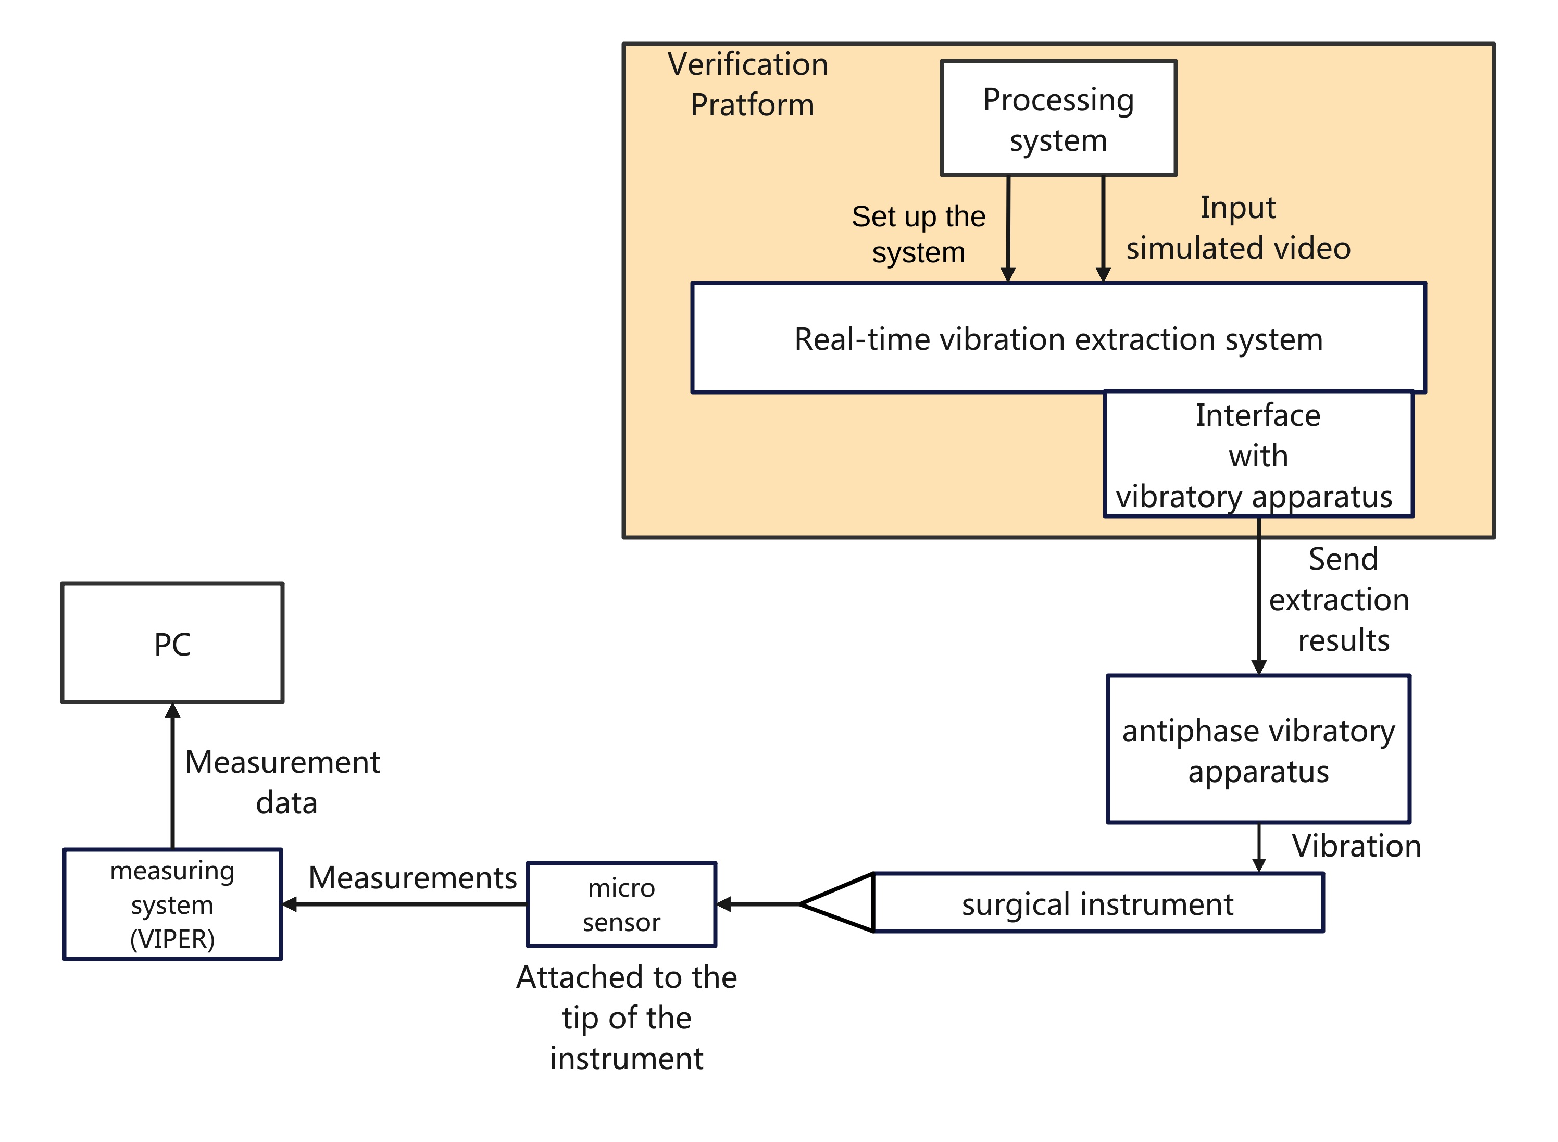
\includegraphics[width = 8cm,pagebox=cropbox,clip]{img/vibration_test.pdf}
  \caption{vibration experiments}
  \label{figure:vibration_test}
\end{figure}


\begin{table}[tb]
  \centering
  \caption{Communication standard with antiphase vibratory apparatus}
  \label{table:interface}
  \begin{tabular}{|c|l|c|}
    %%\toprule
    \hline
    Number & Data & Summary                                         \\ \hline \hline
    %% \midrule
    1 &          0xFF            &   Header                         \\ \hline \hline
    2 & Frame Number( 1〜 8bits) &  Current frame number            \\ \cline{1-2}
    3 & Frame Number( 9〜16bits) &  (Transmitted 8 bits at a time   \\ \cline{1-2}
    4 & Frame Number(17〜24bits) &   starting with the lower bits)  \\ \cline{1-2}
    5 & Frame Number(25〜32bits) &                                  \\ \hline \hline
    6 & Movement Postion( 1〜 8bits)  &  Relative position from the    \\ \cline{1-2}
    7 & Movement Postion( 9〜16bits)  &  start of inhibition ($\mu$m)  \\ \cline{1-2}
    8 & Movement Postion(17〜24bits)  &  (Transmitted 8 bits at a time \\ \cline{1-2}
    9 & Movement Postion(25〜32bits)  &  starting with the lower bits) \\ \hline
    %% \bottomrule
  \end{tabular}
\end{table}



%% この実験では、振動抽出システムと逆位相波加振装置を接続し、
%% 手術器具への加振のテストを行う。
%% この実験の概要を図\ref{figure:vibration_test}に示す。
%% 検証プラットフォームを用いて振動抽出システムに模擬映像を入力する。
%% 抽出結果を加振装置に入力し、手術器具の模型に加振する。
%% その様子を3次元位置測定システムのVIPER\cite{bib:VIPER}を用いて計測する。
%% この計測データを用いて評価を行う。
%% 逆位相波加振装置との通信は表\ref{table:interface}に示す規格に従った。
%% 一回の通信で、ヘッダー、フレームナンバー、手術器具の先端を移動させる位置のデータを送信する。
%% 移動位置は、振動抽出開始時の位置からの相対位置を送信する。

%% この実験を行うにあたり、逆位相波加振装置とのインタフェースをRTLで実装した。
%% 振動抽出システムは1フレームの処理が完了すると、垂直方向の振動成分の抽出結果と、送信開始の信号をインタフェースに入力する。
%% インタフェースは送信開始の信号を受け取ると、表\ref{table:interface}
%% の規格通りにデータを送信する。
%% 今回は位相情報に着目した評価を行うため、振動抽出システムの抽出結果の符号のみを参考に、抽出振動の変位量を固定値(Const\_Value)に変換する。
%% 固定値に変換した抽出データから、抽出データの累積値を計算する。この累積値が振動抽出開始時の位置からの相対位置となる。
%% 次に移動平均フィルタを用いて低周波成分を除去する。
%% これは、予備実験にて累積値が時間の経過とともにマイナス方向にトレンドすることが判明したためである。
%% このトレンド成分を除去するために、ローパスフィルタとして移動平均フィルタ
%% を採用している。
%% 逆位相波加振装置へは、シリアル通信(RS232-C)でデータを送信する。


In this experiment, a vibration extraction system is connected
to a antiphase vibratory apparatus to test the excitation to the surgical instruments.
An overview of this experiment is shown in Figure \ref{figure:vibration_test}.
Input the simulated video to the vibration extraction system using the validation platform.
The extraction results are input to the vibratory apparatus and vibrations are applied to the model of the surgical instrument.
The situation is measured using the electromagnetic motion tracking system, VIPER\cite{bib:VIPER}.
This measurement data is used for evaluation.
The communication with the antiphase vibration apparatus followed the
standard shown in table \ref{table:interface}.
In a single communication, the header, frame number,
and data on the position at which the tip of the surgical instrument is
to be moved are transmitted.
The position to be moved is transmitted relative to the position
at the start of vibration extraction.

To conduct this experiment, an RTL implementation of an interface
to an inverse phase wave excitation system was used.
When the vibration extraction system completes processing one frame,
it inputs the result of the extraction of the vertical vibration
component and the signal to start transmission to the interface.
When the interface receives the signal to start transmission,
it transmits the data as per the standard in the table \ref{table:interface}.
In order to evaluate this time focusing on phase information, the amount of displacement of the extracted vibration is converted to a fixed value (Const\_Value)、with reference only to the sign of
the extraction result of the vibration extraction system.
From the extracted data converted to fixed values,
the cumulative value of the extracted data is calculated.
This accumulated value is the position relative to the position at the start of vibration extraction.
Next, a moving average filter is used to remove low-frequency components.
This is because preliminary experiments have shown that the cumulative values trend
in a negative direction over time, as shown in figure\ref{figure:drift_plot}.
This is because preliminary experiments have shown that the accumulated values trend
in a negative direction over time.
To remove this trend component, a moving average filter is employed as a low-pass filter.
Data is sent to the antiphase vibratory apparatus via serial communication (RS232-C).


\begin{figure}[tb]
  \centering
  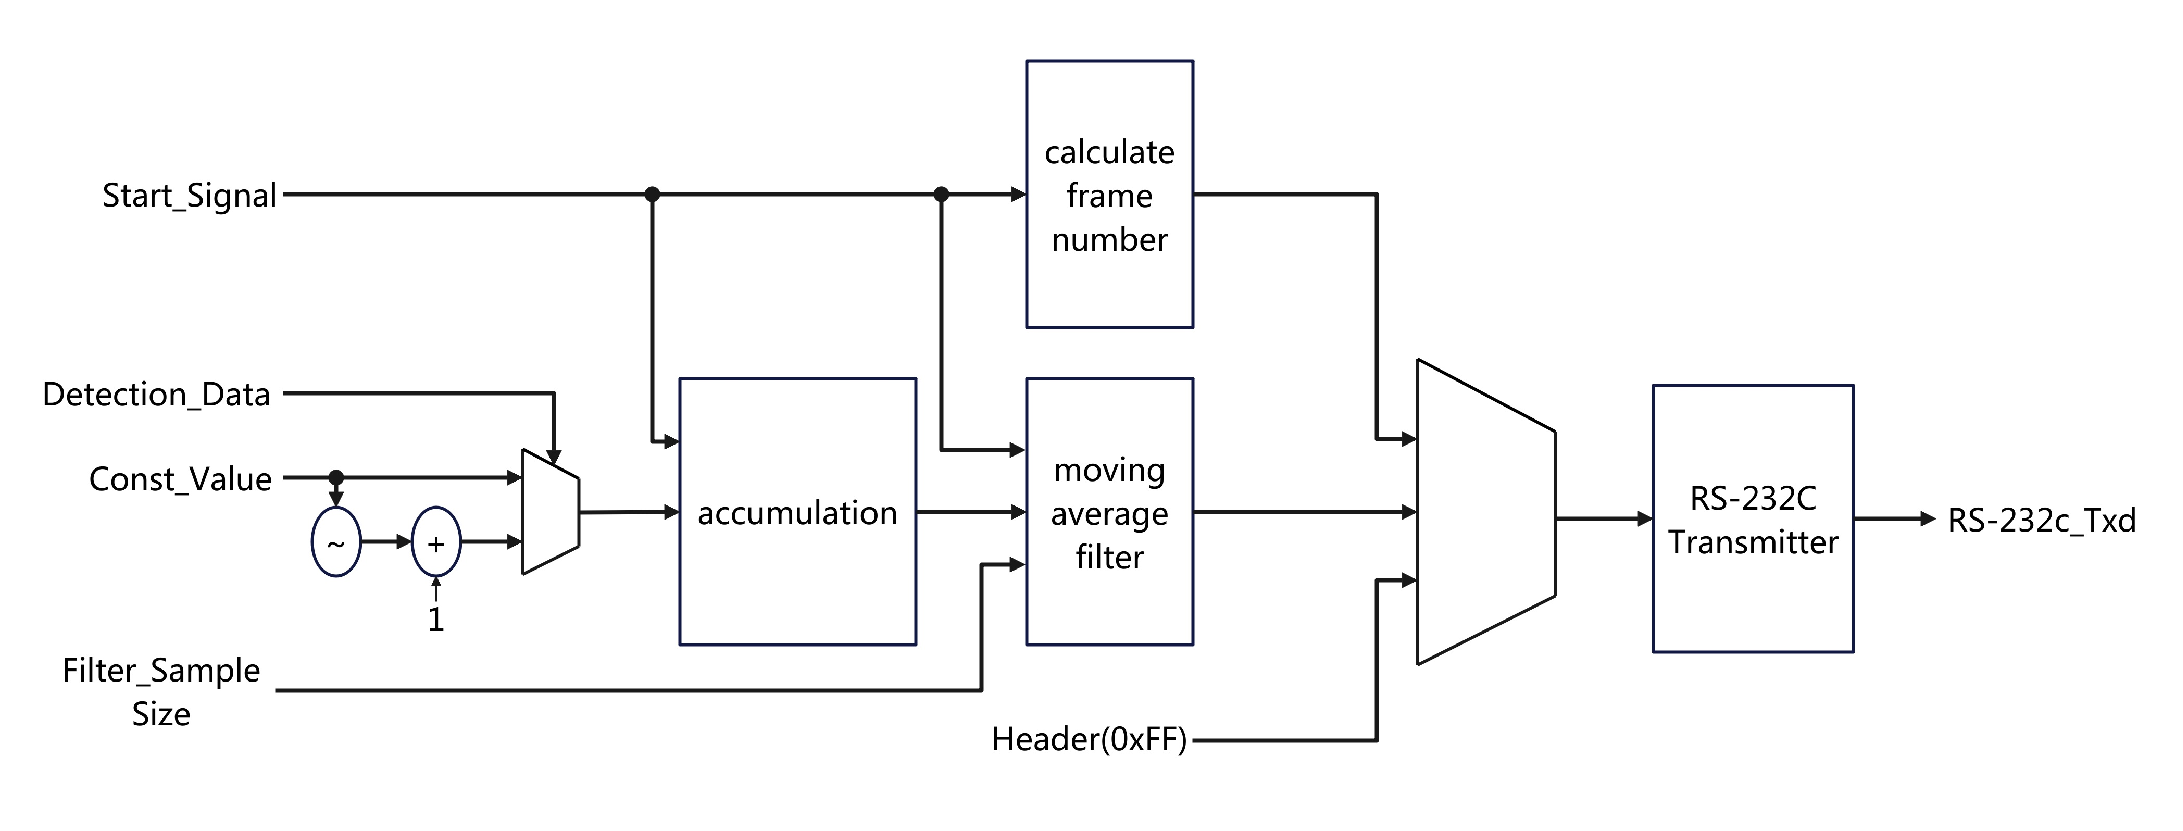
\includegraphics[width = 10cm,pagebox=cropbox,clip]{img/interface.pdf}
  \caption{Interface with vibratory apparatus}
  \label{figure:interface}
\end{figure}

\begin{figure}[tb]
  \centering
  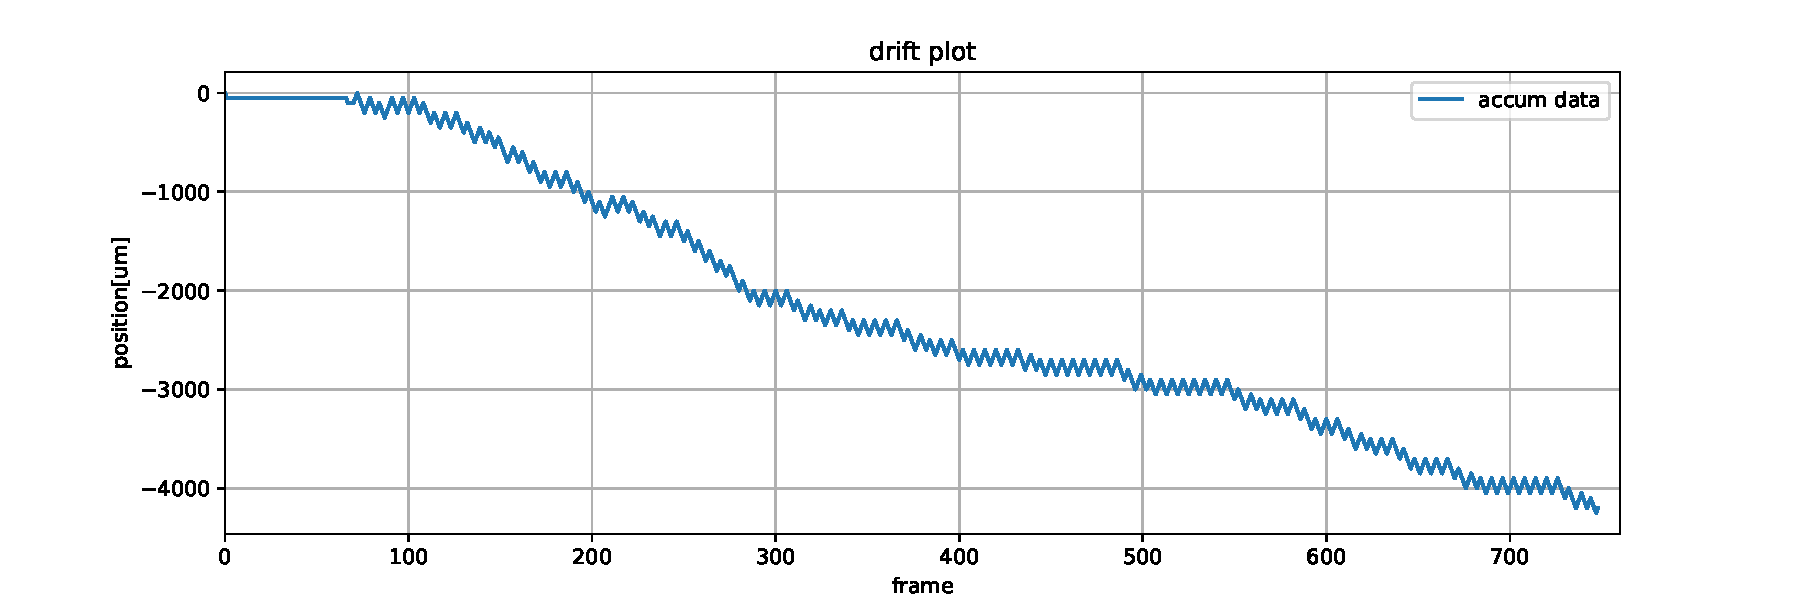
\includegraphics[width = 10cm,pagebox=cropbox,clip]{img/drift_plot.pdf}
  \caption{Cumulative value of extraction results}
  \label{figure:drift_plot}
\end{figure}




\subsection{ Tremor suppression experiment using a tremor reproduction device}\label{subsection:suppression_experiment}

%% この実験では田中らが開発した振戦再現装置\cite{bib:tremor_reproduction}を用いて振戦振動を手術器具に再現し、
%% その振動を振戦抽出システムと逆位相波加振装置を用いて抑制する。
%% 振戦再現装置は手術器具の模型をヒトが手に持った際の手術器具先端の振戦を含む振動を測定し,測定した振動を高精度に再現する.

%% この実験の概要を図\ref{figure:suppression_test}に示す。
%% まず、振戦再現装置を用いて手術器具の模型に振戦振動を再現する。
%% その振動を顕微鏡カメラで捉え、撮影した映像をリアルタイムで振動抽出システムに入力して振戦振動を
%% 抽出する。
%% 抽出した振動情報をもとに逆位相波加振装置で振動抑制を行い、その様子VIPERで計測し評価を行う。


In this experiment, the vibration reproduction device developed by Tanaka et al.\cite{bib:tremor_reproduction_eng}
is used to reproduce the vibration of the surgical instrument,
and the vibration is suppressed using a vibration extraction system and
an antiphase wave apparatus. The vibration reproducer measures vibrations,
including tremors at the tips of surgical instruments when a human holds a model of a surgical instrument in his/her hand,
and reproduces the measured vibrations with high precision. An overview of this experiment is shown in Figure \ref{figure:suppression_test}.
First, vibrations are reproduced on a model of a surgical instrument using a vibration reproduction device. The vibrations are captured by a microscope camera, and the captured images are input to the vibration extraction system real time to extract the vibrations. Based on the extracted vibration information, vibration suppression is performed using an inverse phase wave shaker, and the vibration is measured and evaluated using VIPER.



\begin{figure}[tb]
  \centering
  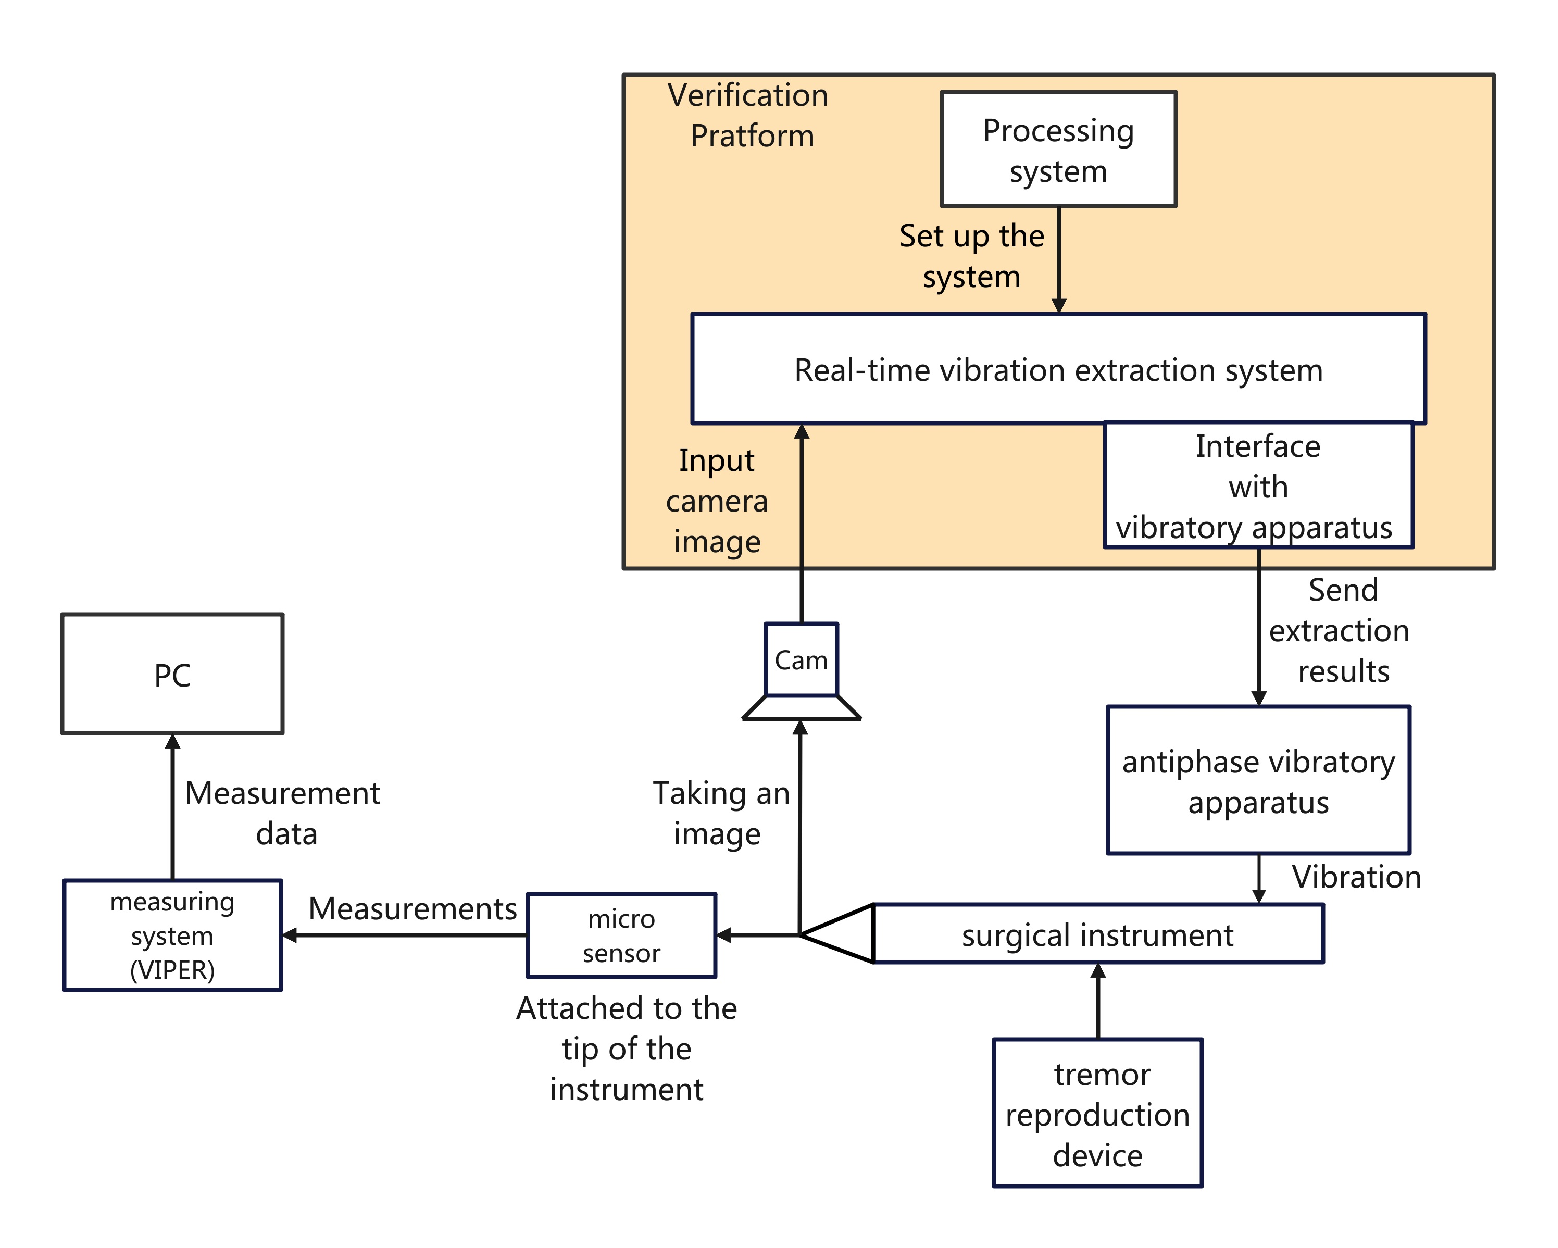
\includegraphics[width = 8cm,pagebox=cropbox,clip]{img/suppression_test.pdf}
  \caption{Cumulative value of extraction results}
  \label{figure:suppression_test}
\end{figure}

\section{Evaluation}\label{section:evaluation}


\subsection{Vibration extraction experiment using simulated video}\label{subsection:eval:experiment1}

\begin{table}[tb]
  \centering
  \caption {Parameters to be evaluated}
  \label{table:bit_eval_parameter1}
  \begin{tabular}{|c|c|}
    %%\toprule
    \hline
    parameter   & value                \\ \hline \hline
    search window size & 11 \\\hline
    cell size   & 9          \\\hline
    %%BMFLCの通過周波数帯の分割数 & 16      \\\hline
    quantization bit width   & 2      \\\hline
     gain parameter of the BMFLC weight vector & $2^{-7}$ \\ \hline
    %%オプティカルフローの閾値   & 1.5                  \\ \hline
  \end{tabular}
\end{table}

%% 表\ref{table:bit_eval_parameter1}に、今回評価する振動抽出システムのパラメータと、
%% パラメータのデフォルト値を示す。

Table \ref{table:bit_eval_parameter1} shows the parameters of the vibration extraction system
to be evaluated in this study and the default values of the parameters.

%% 本研究では、評価指標にWMAPE(Weighted Mean Absolute Percentage Error)と相互相関係数の2つを用いた.
%% WMAPEは眞邉らの研究\cite{bib:Image-Based_Vibration_Extraction}で用いられた評価指標であり,
%% 出力値が真値に近いほど$0$に近い値を示し,出力値がすべて$0$である場合に1を示す.
%% 出力値を$x(k)$,真値を$y(k)$とすると,
%% 以下のように算出される:

Two evaluation indices, WMAPE (Weighted Mean Absolute Percentage Error) and cross-correlation coefficient, were used in this study.
WMAPE is the evaluation index used in the study by Manabe et al.
The closer the output value is to the true value,the closer the value is to $0$, and 1 is indicated when all output values are $0$.
Let $x(k)$ be the output value and $y(k)$ be the true value, and it is calculated as follows:


\begin{equation}
  \label{equ:WMAPE_origin}
  e_{\mathit{norm}} = \frac{\sum_{k} \left| x(k)-y(k) \right| }{\sum_{k} \left| y(k)  \right|}   
\end{equation}


%% 今回の評価では位相情報に着目した評価を行うため,$x(k)$,$y(k)$を独立に正規化するように変更した式を使用した:

In this evaluation,
we used the modified equation to normalize $x(k)$ and $y(k)$ independently in order to focus on the phase information:


\begin{equation}
  \label{equ:WMAPE}
  e_{\mathit{scale}} =  \sum_{k}  \left| \frac{\sum_{k} x(k)}{\sum_{k} |x(k)|}  - \frac{\sum_{k} y(k)}{\sum_{k} |y(k)|} \right|    
\end{equation}


%% また,相互相関係数とは$x(k)$,$y(k)$のそれぞれの分散$S_x$,$S_y$と共分散$S_{xy}$から,
%% で求められる評価指標である.
%% 正の相関が強いほど$1$に近い値を示し,負の相関が強いほど$-1$に近い値を示す評価関数である.
%% 相関がない場合は$0$に近い値を示す.
%% 相互相関係数は以下のように求められる。

The cross-correlation coefficient is an evaluation index calculated from the variance $S_x$, $S_y$
and covariance $S_{xy}$ of $x(k)$ and $y(k)$, respectively.
The stronger the positive correlation, the closer the value to $1$, and the stronger the negative correlation,
the closer the value to $1$. When there is no correlation,
the value is close to $0$. The cross-correlation coefficient is obtained as follows:

\begin{equation}
  \label{equ:cross-correlation}
  r= \frac{s_{xy}}{s_xs_y}
  =\frac{\frac{1}{n} \sum_{i=0}^{n}(x_i - \bar{x})(y_i - \bar{y})}
  {\sqrt{\frac{1}{n} \sum_{i=0}^{n}(x_i-\bar{x})^2}\sqrt{\frac{1}{n} \sum_{i=0}^{n}(y_i-\bar{y})^2}}    
\end{equation}



%% なお,適応推定フィルタであるBMFLCは適応するまでに一定の時間を要するため,$750$フレームのデータのうち,
%% $300$フレームから$750$フレームの出力値を評価対象とした.

Since the adaptive estimation filter, BMFLC, takes a certain amount of time to adapt,
the output values from $300$ to $750$ frames out of $750$ frames of data were the target of evaluation.


%% まずはじめに、オプティカルフローの探索ウインドウサイズを変化させた際の出力値の評価結果を表\ref{table_window_size}示す。
%% ウインドウサイズが大きくなるほどWMAPEの値は低下し,相互相関係数の値が上昇していることがわかる.
%% このことから,ウインドウサイズを大きくすることが抽出精度の向上に効果的であることが分かった.

First of all, the results of the evaluation of the output values when the optical flow search window size is
varied are shown in Table \ref{table:window_size}.
It can be seen that as the window size increases,
the value of WMAPE decreases and the value of the cross-correlation coefficient increases.
This indicates that increasing the window size is effective in improving the extraction accuracy.


\begin{table}[tb]
  \centering
  \caption{Evaluation results when search window size is varied}
  \label{table:window_size}
  \begin{tabular}{|c|c|c|}
    %%\toprule
    \hline
    search window size   & WMAPE &cross correlation  \\ \hline \hline
    9         &1.42930  &0.31552       \\ \hline
    11        &0.76671  &0.66365 \\ \hline
    13        &0.67171  &0.73732 \\ \hline
    15        &0.64146  &0.76056  \\ \hline
    17        &0.54591  &0.82015  \\ \hline
    19        &0.49598  &0.84790   \\ \hline
    21        &0.42631  &0.87880  \\ \hline
    23        &0.40533  &0.88938   \\ \hline
    25        &0.37493  &0.90636  \\ \hline
    27        &0.35800  &0.91632   \\ \hline
  \end{tabular}
\end{table}




%% 次に,セルサイズを変化させた場合の評価を行った.ウインドウサイズは先ほどの評価で最も抽出精度が高かった
%% 27を使用し,その他のパラメータはパラメータ群1の値に固定した.
%% 各セルサイズにおける評価結果を表\ref{table:cell_size}に示す.
%% ウインドウサイズ同様に,セルサイズが大きくなるほどWMAPEの値は低下し,相互相関係数の値が上昇していることがわかる.
%% このことから,セルサイズを大きくすることが抽出精度の向上に効果的であることが分かった.


Next, the evaluation was conducted for varying cell size.
The search window size was set to $27$, which had the highest extraction accuracy in the previous evaluation.
The evaluation results for each cell size are shown in Table \ref{table:cell_size}.
As with the search window size, it can be seen that as the cell size increases,
the value of WMAPE decreases and the value of the cross-correlation coefficient increases.
This indicates that increasing the cell size is effective in improving the extraction accuracy.


\begin{table}[tb]
 \centering
 \caption{Evaluation results when cell size is varied}
 \label{table:cell_size}
 \begin{tabular}{|c|c|c|}
   %%\toprule
   \hline
   cell size & WMAPE &cross correlation \\ \hline \hline
   9         &0.35799  &0.91632       \\ \hline
   11        &0.34619  &0.92174 \\ \hline
   13        &0.33681  &0.92742 \\ \hline
   15        &0.32301  &0.93433  \\ \hline
   17        &0.32081  &0.93625  \\ \hline
   19        &0.32086  &0.93686   \\ \hline
   21        &0.31727  &0.93987  \\ \hline
   23        &0.31078  &0.94436   \\ \hline
   25        &0.30074  &0.94905   \\ \hline
   27        &0.28922  &0.95342 \\ \hline
 \end{tabular}
\end{table}



%% 次に,BMFLCの適応ゲインパラメータを変化させた場合の評価を行った.
%% 各ゲインパラメータにおける評価結果を表\ref{table:gain}に示す.
%% ゲインパラメータを大きくすると,収束速度が向上する半面,安定性が損なわれ,WMAPEの値は大きく,相互相関係数の値は小さい.
%% また,ゲインパラメータを小さくすると安定性が向上する半面,収束速度が低下し,300フレームからの750フレームの評価では
%% 抽出精度が低下する傾向があることが分かった.


Next, we evaluated the BMFLC when the adaptive gain parameters were varied.
The evaluation results for each gain parameter are shown in Table \ref{table:gain}.
As the gain parameter is increased, the convergence speed increases, but stability is impaired,
and the WMAPE value is larger and the cross-correlation coefficient is smaller.
When the gain parameter is decreased, the stability improves, but the convergence speed decreases,
and the extraction accuracy tends to decrease for the evaluation of 750 frames from 300 frames.


\begin{table}[tb]
  \centering
  \caption{Evaluation results when gain parameter is varied}
  \label{table:gain}
  \begin{tabular}{|c|c|c|}
    %%\toprule
    \hline
    gain parameter   & WMAPE & cross correlation     \\ \hline \hline
    $2^{-3}$        &1.29598 &0.04524       \\ \hline
    $2^{-4}$        &1.36716  & -0.0142 \\ \hline
    $2^{-5}$        &0.97749  &0.53896 \\ \hline
    $2^{-6}$       &0.32301  &0.88169  \\ \hline
    $2^{-7}$        &0.28922  &0.95342  \\ \hline
    $2^{-8}$        &0.22523  &0.97019   \\ \hline
    $2^{-9}$        &0.22797  &0.968040  \\ \hline
    $2^{-10}$       &0.27036  &0.947585  \\ \hline
  \end{tabular}
\end{table}


%% 最後に、勾配方向の量子化ビット幅を変化させた際の出力値の評価を行った。
%% その他のパラメータについて、表\ref{table:quan_param}に示す2パターンのパラメータ群を用意し、
%% それぞれのパターンの量子化ビット幅を変更する。
%% 各パターンにおける評価結果を表\ref{table:quan}に示す。
%% パターン$1$においては量子化ビット幅を大きくするほど抽出精度が良くなっているが、
%% パターン$2$においては、量子化ビット幅を大きくするほど抽出精度が悪くなっていることがわかる。
%% この結果から、量子化ビット幅はその他のパラメータによって,適した値が変わることがわかった。


Finally, the output values were evaluated when the quantization bit width in the gradient direction was varied.
For the other parameters, we prepared a group of parameters for the two patterns shown in Table \ref{table:quan_param}
and changed the quantization bit width for each pattern.
The evaluation results for each pattern are shown in table\ref{table:quan_param}.
It can be seen that in pattern $1$,the extraction accuracy improves as the quantization bit width is increased,
while in pattern $2$, the extraction accuracy worsens as the quantization bit width is increased.
This result indicates that the appropriate value of the quantization bit width varies depending on other parameters.


\begin{table}[tb]
  \centering
  \caption {Parameters to be evaluated}
  \label{table:quan_param}
  \begin{tabular}{|c|c|c|}
    %%\toprule
    \hline
    parameter                & pattern 1 & pattern2 \\ \hline \hline
    search window size       &   9       &   19 \\\hline
    cell size                &   9       &   19 \\\hline
    gain parameter of the BMFLC weight vector & $2^{-7}$ & $2^{-7}$  \\ \hline
  \end{tabular}
\end{table}



\begin{table}[tb]
  \centering
  \caption{Evaluation results when quantization bit width}
  \label{table:quan}
  \begin{tabular}{|c|c|c|c|}
    %%\toprule
    \hline
    pattern & quantization bit width   & WMAPE & cross correlation     \\ \hline \hline
    1       &  1         &1.98376   &  0.05763       \\ \hline
    1       &  2         &1.42930   &  0.31552    \\ \hline
    1       &  3         &1.20372   &  0.36329 \\ \hline
    2       &  1         &0.39431   &  0.89721  \\ \hline
    2       &  2         &0.47363   &  0.85405  \\ \hline
    2       &  3         &0.48867   &  0.84429   \\ \hline
  \end{tabular}
\end{table}






\subsection{Vibration experiments using a vibratory apparatus}\label{subsection:eval:add_experiment}

\begin{table}[tb]
  \centering
  \caption{Parameters of the system during the vibration experiment}
  \label{bit_table:vibration_parameter}
  \begin{tabular}{|c|c|}
    %%\toprule
    \hline
    parameter   & value                \\ \hline \hline
    search window size & 27 \\\hline
    cell size   & 27          \\\hline
    %%BMFLCの通過周波数帯の分割数 & 16      \\\hline
    quantization bit width   & 2      \\\hline
    gain parameter of the BMFLC weight vector & $2^{-7}$ \\ \hline
    %%オプティカルフローの閾値   & 1.5                  \\ \hline
  \end{tabular}
\end{table}


%% 表\ref{bit_table:vibration_parameter}に加振実験を行った際の振動抽出FPGAシステムのパラメータを示す.
%% 図\ref{figure:supp_eval:vibration_test_result},図\ref{figure:supp_eval:vibration_test_result_fft}に
%% 加振実験の結果を示す.
%% 図\ref{figure:supp_eval:vibration_test_result}は,縦軸が移動位置,横軸が時間の波形であり,約$1.3 \sim 4.5$秒間
%% にズームした図である.オレンジ線がインタフェースが出力した値,青線がVIPERで測定した加振実験の結果である.
%% また,図\ref{figure:supp_eval:vibration_test_result_fft}は図\ref{figure:supp_eval:vibration_test_result}の結果の
%% 振幅スペクトルである.

%% 図\ref{figure:supp_eval:vibration_test_result},
%% 図\ref{figure:supp_eval:vibration_test_result_fft}の通り,
%% 逆位相波発生装置の加振結果には,インタフェースが出力した
%% 振動データに含まれない振動成分が含まれていることがわかった.
%% そのため,逆位相波発生装置が振動抽出FPGAシステムの振動データを
%% 正確に加振できているとは言えない結果となった.


Table \ref{bit_table:vibration_parameter} shows the parameters of the vibration extraction system during the shaker experiments.
Figure\ref{figure:supp_eval:vibration_test_result} and Figure\ref{figure:supp_eval:vibration_test_result_fft} show
the results of the shaking experiment. Figure\ref{figure:supp_eval:vibration_test_result} shows the waveform with
the vertical axis representing the moving position and the horizontal axis representing time,
zoomed in for about $1.3 \sim 4.5$ seconds.
The figure is zoomed to about $1.3 \sim 4.5$s.
The orange line is the value output by the interface.
The orange line is the value output by the interface, and the blue line is the result of the vibration experiment measured by VIPER.
Figure\ref{figure:supp_eval:vibration_test_result_fft} is the amplitude spectrum of the result of Figure \ref{figure:supp_eval:vibration_test_result}.
shown in Figures \ref{figure:supp_eval:vibration_test_result} and \ref{figure:supp_eval:vibration_test_result_fft},
the vibration results of the antiphase vibratory apparatus include vibration components that are not included
in the vibration data output by the interface.
Therefore, it cannot be said that the antiphase vibratory apparatus accurately excites the
vibration data of the vibration extraction FPGA system.



\begin{figure}[tb]
  \centering
  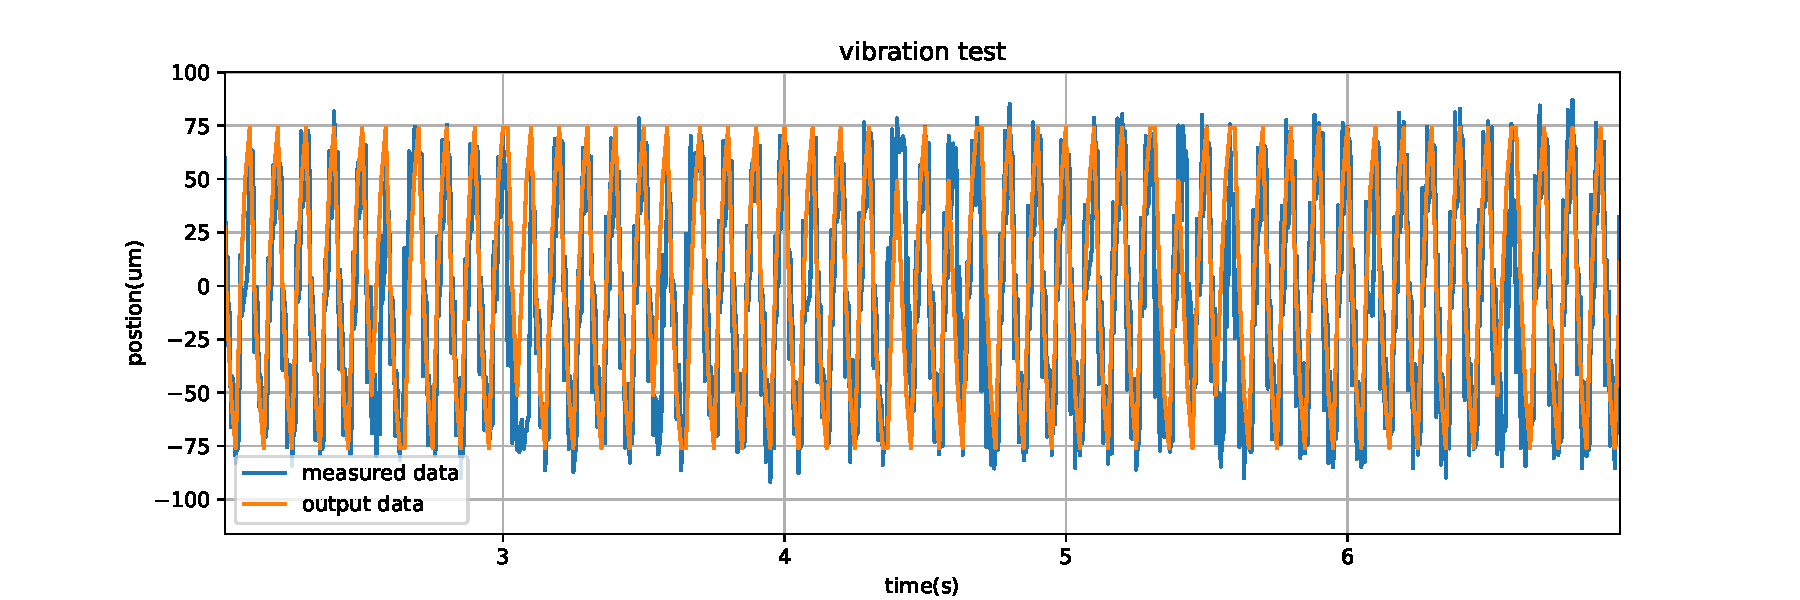
\includegraphics[width = 10cm,pagebox=cropbox,clip]{img/Supdevice_result.pdf}
  \caption{result:vibration experiment}
  \label{figure:supp_eval:vibration_test_result}
\end{figure}

\begin{figure}[tb]
  \centering
  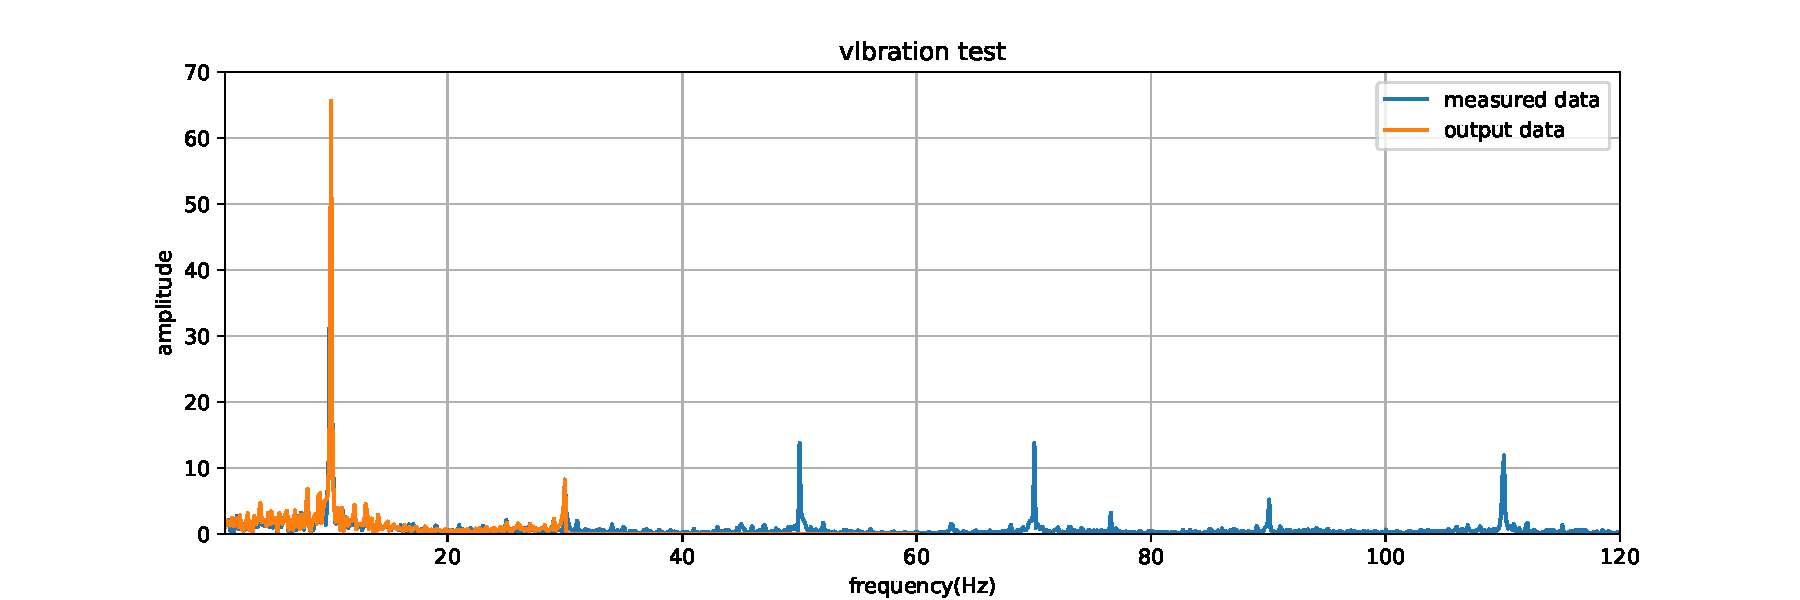
\includegraphics[width = 10cm,pagebox=cropbox,clip]{img/Supdevice_result_fft.pdf}
  \caption{spectrum:vibration experiment}
  \label{figure:supp_eval:vibration_test_result_fft}
\end{figure}








\subsection{ Tremor suppression experiment using a tremor reproduction device}\label{subsection:eval:suppression_experiment}

%% 抑制実験の結果を図\ref{figure:saupp_eval:10Hz_supp}に示す.
%% また,抑制結果の振幅スペクトルを図\ref{figure:saupp_eval:10Hz_supp_fft}に示す.
%% 図\ref{figure:saupp_eval:10Hz_supp}からわかるように,振幅の低下と
%% 増大が周期的に現れていることがわかる.


The results of the suppression experiment are shown in Figure\ref{figure:saupp_eval:10Hz_supp}.
The amplitude spectrum of the suppression results is shown in Figure\ref{figure:saupp_eval:10Hz_supp_fft}.
As can be seen from Figure\ref{figure:saupp_eval:10Hz_supp},
the amplitude decreases and increases periodically.


  \begin{figure}[tb]
    \centering
    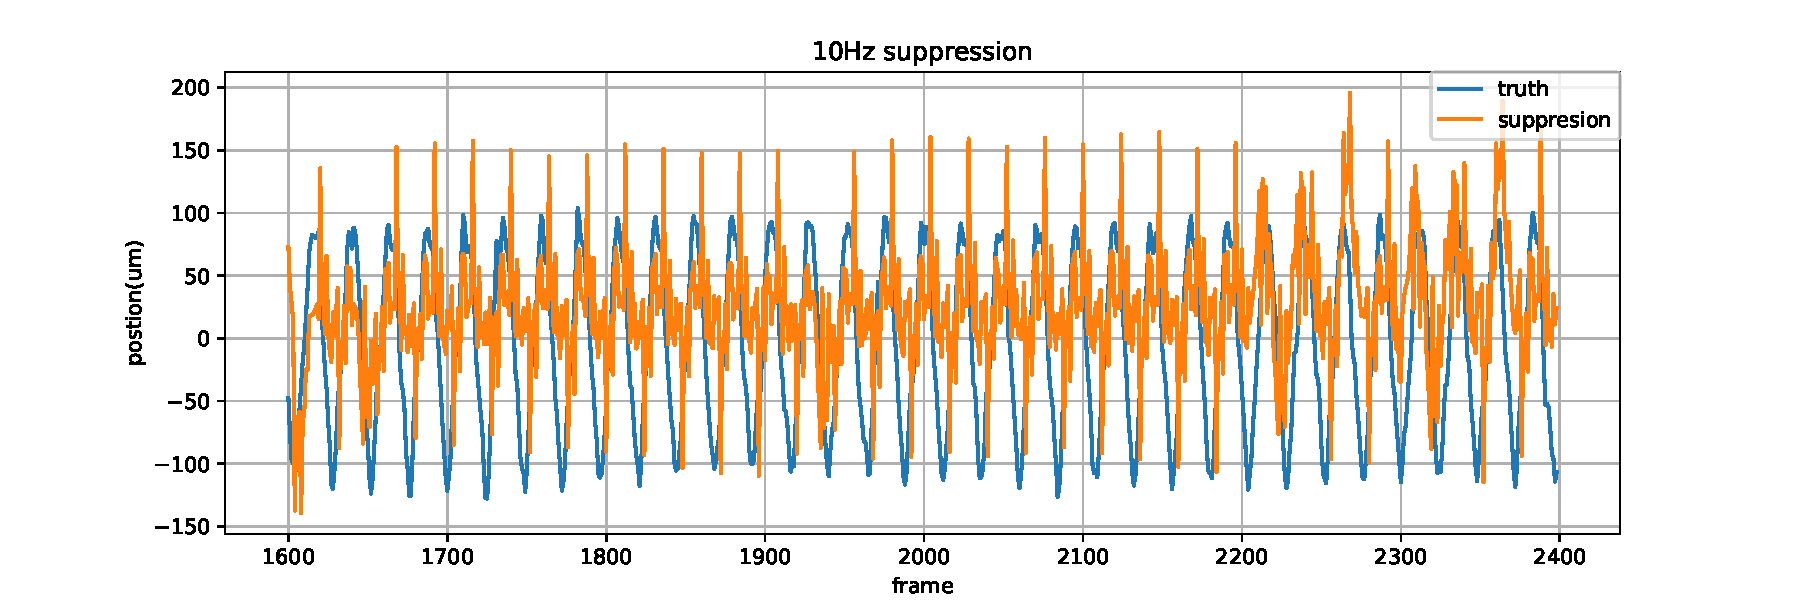
\includegraphics[width = 10cm,pagebox=cropbox,clip]{img/suppression_result.pdf}
    \caption{result:tremor suppression experiment}
    \label{figure:saupp_eval:10Hz_supp}
  \end{figure}
  
  \begin{figure}[tb]
    \centering
    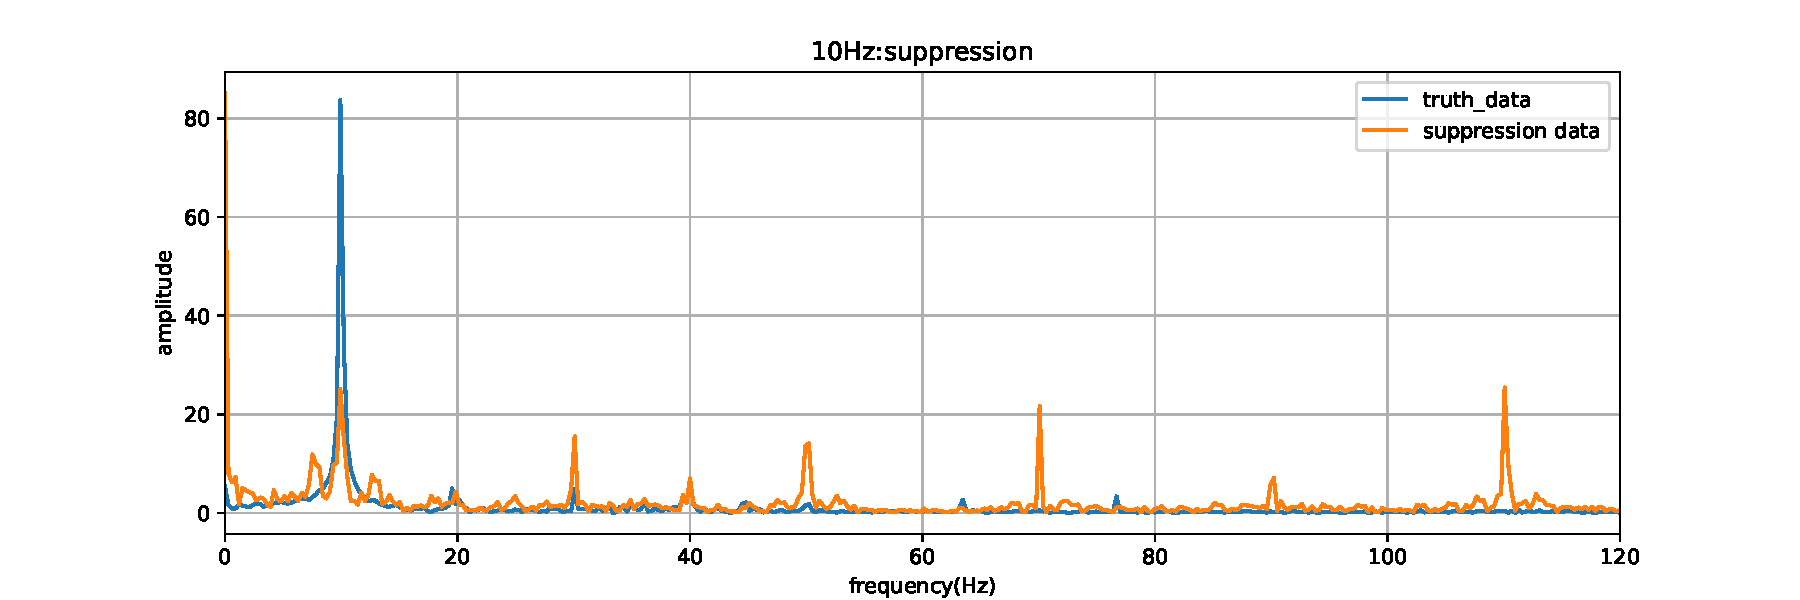
\includegraphics[width = 10cm,pagebox=cropbox,clip]{img/suppression_result_fft.pdf}
    \caption{spectrum:tremor suppression experiment}
    \label{figure:saupp_eval:10Hz_supp_fft}
  \end{figure}

\section{Conclusion}\label{section:conclusion}

%% 本論文では三つの実験を行い、眞邊らが開発したリアルタイム振動抑制システムの
%% 抽出精度と振戦抑制の評価を行った。
%% 検証プラットフォームを用いた振動抽出実験では、
%% オプティカルフローの探索ウインドウサイズやセルサイズを大きくすることが
%% 振動の抽出精度の向上に効果的であることがわかった。
%% また、BMFLCの重みの収束速度を調整するゲインパラメータは、
%% 今回の評価においては、$2^{-7}$,$2^{-8}$,$2^{-9}$が適切であることが分かった。

%% 逆位相波加振装置を用いた加振実験では、意図しない周波数成分が逆位相波加振装置
%% の加振振動に含まれることがわかった。
%% 最後に行った制振実験では,振戦振動の周波数成分の低下がみられたが,
%% 意図しない周波数成分の影響などにより,
%% その他の周波数成分の振動成分が増加が認められた.

%% 今後の課題として,逆位相波発生装置において,意図しない周波数成分が発生する原因の解明や,非定常振動における振戦の制振評価,
%% 振動の変位量を高精度で推定可能なアルゴリズムの検討を行う.


In this paper, three experiments were conducted to evaluate the extraction accuracy
and tremor suppression of the real-time vibration extraction system of Manabe et al.

Vibration extraction experiment
Vibration extraction experiments using the validation platform showed that
increasing the optical flow search window size and cell size was effective in improving
vibration extraction accuracy.
The gain parameters that adjust the convergence speed of the BMFLC weights
were found to be $2^{-7}$, $2^{-8}$, and $2^{-9}$ appropriate for the current evaluation.

In the vibration experiments using a antiphase vibratory apparatus,
it was found that an unintended frequency component was included in the excitation vibration
of the antiphase vibratory apparatus.

In the Tremor suppression experiment using a tremor reproduction device,
a decrease in the frequency component of the excitation vibration was observed,
but an increase in the vibration component of other frequency components
was observed due to the influence of unintended frequency components and other factors.


Future work includes clarifying the causes of unintended frequency components
in antiphase vibratory apparatus, evaluating vibration control in unsteady vibration,
and studying algorithms that can estimate vibration displacements with high precision.


\section{Ackhowledgment}\label{section:ackhowledgment}
Acknowledgments are omitted for double-blind review.


%% \bibliographystyle{jplain}
\bibliographystyle{style/IEEEtran.bst}
%% \bibliography{bib/0-refs.bib}
\bibliography{bib/99-refs.bib}

\end{document}
